\section{Sentiment Analysis}
\label{sec:analysis}

Sentiment analysis is an interdisciplinary field
that crosses natural language processing (NLP),
artificial intelligence, and text mining~\cite{Dri18}.
It is also called \emph{opinion mining} and its main purpose is
to analyse people's opinions, sentiments, evaluations, appraisals, attitudes, and emotions towards entities such as products, services,
organisations, individuals, issues, events, topics, and their attributes.
Sentiment analysis represents a large problem space.

There are also many names and slightly different tasks
such as \emph{sentiment analysis, opinion mining, opinion extraction, sentiment mining, subjectivity analysis, affect analysis, emotion analysis,
review mining}.
However, they are now all under the umbrella
of sentiment analysis or opinion mining.
While in industry, the term \emph{sentiment analysis} is more commonly used,
in academia both \emph{sentiment analysis}
and \emph{opinion mining} are frequently employed.
Regardless, they basically represent the same field of study,
and mainly focus on opinions
which express or imply positive or negative sentiments.

Although linguistics and NLP have a long history,
little research had been done about people's opinions and sentiments
before the year 2000.
Since then, the field has become a very active research area.
There are several reasons for this.
First, it has a wide arrange of applications, almost in every domain.
The industry surrounding sentiment analysis has also flourished
due to the proliferation of commercial applications.
This provides a strong motivation for research.
Second, it offers many challenging research problems,
which had never been studied before.
Third, for the first time in human history,
we now have a huge volume of opinionated data in the social media on the Web. Without this data, a lot of research would not have been possible~\cite{Liu12}.

Not surprisingly, the inception and rapid growth of sentiment analysis coincide with those of the social media.
In fact, sentiment analysis is now right at the centre
of the social media research.
Hence, research in sentiment analysis not only has an important impact on NLP, but may also have a profound impact on management sciences,
political science, economics, and social sciences
as they are all affected by people's opinions.
Although the sentiment analysis research mainly started from early 2000,
there was some earlier work on interpretation of metaphors,
sentiment adjectives, subjectivity, view points, and affects~\cite{HM97,Hea92,WBO99}.

\subsection{Levels}
\label{subsec:levels}

In general,
sentiment analysis has been investigated mainly at three levels
which are described further on.

\begin{itemize}
 \item \textbf{Document level}: The task at this level is
 to classify whether a whole opinion document expresses a positive or negative sentiment~\cite{PLV02}.
 For example, given a product review, the system determines
 whether the review expresses an overall positive or negative opinion
 about the product.
 This task is commonly known as \emph{document-level sentiment classification}. This level of analysis assumes that each document expresses opinions
 on a single entity (e.g., a single product).
 Thus, it is not applicable to documents which evaluate
 or compare multiple entities.
 
 \item \textbf{Sentence level}: The task at this level goes to the sentences
 and determines whether each sentence expressed a positive, negative,
 or neutral opinion.
 Neutral usually means no opinion.
 This level of analysis is closely related
 to \emph{subjectivity classification}~\cite{WBO99},
 which distinguishes sentences (called \emph{objective sentences})
 that express factual information
 from sentences (called \emph{subjective sentences})
 that express subjective views and opinions.
 However, we should note that subjectivity is not equivalent to sentiment
 as many objective sentences can imply opinions,
 e.g., \emph{``We bought the car last month
 and the wind shield wiper has fallen off.''}.
 
 \item \textbf{Entity and Aspect level}: Both the document-level
 and sentence-level analyses do not discover
 what exactly people liked and did not like.
 Aspect level performs finer-grained analysis.
 Instead of looking at language constructs
 (documents, paragraphs, sentences, clauses, or phrases),
 aspect level directly looks at the opinion itself.
 It is based on the idea that an opinion consists
 of a \emph{sentiment} (positive or negative) and a \emph{target} (of opinion).
 In many applications,
 opinion targets are described by entities and/or their different aspects.
 Thus, the goal of this level of analysis is
 to discover sentiments on entities and/or their aspects.
 For example, the sentence
 \emph{``The iPhone's call quality is good, but its battery life is short.''} evaluates two aspects:
 \emph{call quality} and \emph{battery life}, of iPhone (entity).
 The sentiment on iPhone's \emph{call quality} is positive,
 but the sentiment on its \emph{battery life} is negative.
 The \emph{call quality} and \emph{battery life}
 of iPhone are the opinion targets.
 Based on this level of analysis,
 a structured summary of opinions about entities and their aspects
 can be produced, which turns unstructured text to structured data
 and can be used for all kinds of qualitative and quantitative analyses.
\end{itemize}

Both the document-level and sentence-level classifications
are highly challenging and often insufficient for applications
because they do not identify opinion targets
or assign sentiments to such targets.
Even if we assume that each document evaluates a single entity,
a positive opinion document about the entity does not mean
that the author has positive opinions about all aspects of the entity.
Likewise, a negative opinion document does not mean
that the author is negative about everything.
For more complete analysis, we need to discover the aspects
and determine whether the sentiment is positive or negative on each aspect.
Therefore, the aspect-level seems a more favourable practice but still,
it is even more difficult to implement
and also consists of several sub-problems
as explained in the work of Liu~\cite{Liu12}
on sentiment analysis and opinion mining.

\subsection{Features}
\label{subsec:features}

In the field of sentiment analysis,
the unit of text may be represented by specific features.
Abbasi et al.~\cite{ACS08} in their study on feature selection
for opinion classification in web forums
list four categories of such features.
These include \emph{syntactic}, \emph{semantic}, \emph{link-based},
and \emph{stylistic} features,
and are further elaborated below.

\begin{itemize}
 \item \textbf{Syntactic features}:
 These include word \emph{n}-grams, part-of-speech (POS) tags, and punctuation.
 Additionally, they may include phrase patterns
 which make use of POS tag \emph{n}-gram patterns.
 Along with semantic features,
 syntactic attributes are the most commonly used set of features
 for sentiment analysis~\cite{ACS08}.
 
 \item \textbf{Semantic features}:
 These incorporate manual, semi-automatic,
 or fully automatic annotation techniques to add polarity (positive/negative),
 or affect intensity-related scores to words and phrases.
 Sentiment lexicons with annotated positive, negative
 and sometimes objective terms are usually deployed for that purpose.
 Other semantic attributes include contextual features
 representing the semantic orientation of surrounding text,
 which have been useful for sentence-level sentiment classification.
 
 \item \textbf{Link-based features}:
 These refer to link/citation analysis
 for the evaluation of sentiments for Web artefacts and documents.
 Efron~\cite{Efr08} in his work
 on classifying subjective documents by cociation analysis
 discovered that opinion Web pages heavily linking to each other
 often share similar sentiments.
 However, due to the limited usage of link-based features,
 it is unclear how effective link-based features may be
 for sentiment classification~\cite{ACS08}.
 
 \item \textbf{Stylistic features}:
 These include lexical and structural attributes such as
 the frequency of letters (e.g. a, b, c),
 the use of special characters (@\#\$\%\&*\^{}),
 and the sentence length.
 However, lexical and structural style markers have seen limited usage
 in sentiment analysis research~\cite{ACS08}. 
\end{itemize}

Due to the selection of a large amount of features,
researchers often resort to feature selection prior to classifier calibration,
to identify and use the most significant discriminators of
opinion expression for each case~\cite{GSZ13,ACS08,Gam04}.

\subsection{Approaches}
\label{subsec:approaches}

The widespread approaches of sentiment analysis can be broadly categorised
into two main classes according to the work of Dritsa~\cite{Dri18}.
These classes are depicted in the following figure.

\begin{figure}[ht]
\centering
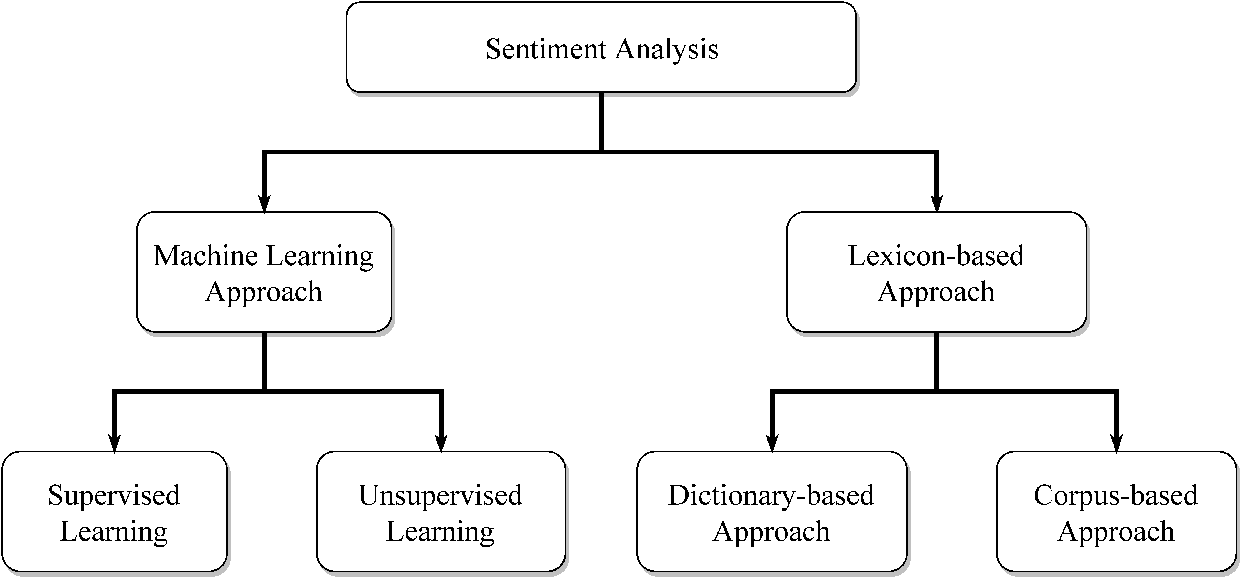
\includegraphics[width=\textwidth]{approaches.eps}
\caption{Sentiment Analysis Approaches}
\label{fig:approaches}
\end{figure}

\clearpage

\begin{itemize}
 \item \textbf{Machine Learning approach}:
 The first class of approaches utilises a textual feature representation
 mixed with machine learning algorithms
 to derive the relationship between features of the text segment
 and the opinions expressed in the writing,
 in either a \emph{supervised} or an \emph{unsupervised} way~\cite{GSZ13,PLV02}.
 With the term \emph{supervised},
 we mean that the classifier receives a set of manually labelled examples
 as training data and makes predictions for all unseen points~\cite{MRT12}.
 With the term \emph{unsupervised},
 we mean that the classification algorithm receives unlabelled data
 and makes evaluations or predictions for all unseen points~\cite{MRT12}.
 Labels can be assigned to training instances manually
 through human evaluation of the text, or can be predefined with ratings
 such as the number of stars in a review~\cite{GSZ13}.
 \emph{Semi-supervised} and \emph{unsupervised} techniques are proposed
 when there is no initial set of labelled data
 for training the classification algorithm~\cite{HZ11,XGYZ13}.
 Furthermore, \emph{hybrid} approaches,
 combining \emph{supervised} and \emph{unsupervised} techniques,
 or even \emph{semi-supervised} techniques,
 can be used to classify sentiments~\cite{KL14,KB06}.
 Concerning the feature selection for the detection of sentiment,
 Natural Language Processing plays an important role
 as it provides useful commonly used features
 such as the frequency of terms, part-of-speech information
 and syntactic dependencies~\cite{SORH15}.
 
 Many prominent approaches to sentiment analysis utilise
 machine learning techniques to develop classifiers~\cite{DLP03,PLV02,ACS08,Gam04}.
 Among the various machine learning techniques,
 Support-Vector Machines (SVMs) and Na\"{i}ve Bayes are most commonly
 applied~\cite{SORH15,GSZ13,PLV02}.
 The use of deep learning, artificial neural networks
 (such as Convolutional Neural Networks (CNN)
 and Long Short-Term Memory (LSTM) networks)
 and maximum entropy models have also demonstrated success
 in sentiment analysis applications, gaining more and more popularity~\cite{GSZ13}.
 Support Vector Machines are also combined with neural network methods
 or with dense word embedding features~\cite{RFN17,GSZ13}.
 
 \item \textbf{Lexicon-based approach}:
 The second class bases the evaluation of a text on a sentiment lexicon
 of opinion-related and usually manually defined positive or negative terms
 in an unsupervised way~\cite{SORH15,GSZ13,Tur02}.
 In this class, one can find two subcategories:
 the dictionary-based approach,
 where the analysis is based on the use of an initial set of terms
 that are usually manually collected and annotated,
 and the corpus-based approach, where the analysis is based
 on domain-related dictionaries.
 These dictionaries are generated from a set of terms
 that grows through the search of related words
 with statistical or semantic techniques~\cite{SORH15}.
 
\end{itemize}

In this thesis we focus on the lexicon-based approach.
We analyse its characteristics, advantages and related work
implemented first for all languages and then exclusively for the Greek.
We also propose a specific methodology for the Greek language
that deploys the dictionary-based approach in Section~\ref{sec:methodology}
and later implement it in Part II: Section~\ref{sec:results}.
